%中間審査概要テンプレート ver. 3.0

\documentclass[uplatex,twocolumn,dvipdfmx]{jsarticle}
\usepackage[top=22mm,bottom=22mm,left=22mm,right=22mm]{geometry}
\setlength{\columnsep}{10mm}
\usepackage[T1]{fontenc}
\usepackage{txfonts}
\usepackage[expert,deluxe]{otf}
\usepackage[dvipdfmx,hiresbb]{graphicx}
\usepackage[dvipdfmx]{hyperref}
\usepackage{pxjahyper}
\usepackage{secdot}





%タイトルと学生番号,名前だけ編集すること
\title{\vspace{-5mm}\fontsize{14pt}{0pt}\selectfont 研究タイトル}
\author{\normalsize プロジェクトマネジメントコース 矢吹研究室 1234567 氏名}
\date{}
\pagestyle{empty}
\begin{document}
\fontsize{10.5pt}{\baselineskip}\selectfont
\maketitle





%以下が本文
\section{背景}

矢吹研究室では課題研究のレジュメは\LaTeX で書くことになっている.

\noindent
□□□□□□□□□■□□□□□□□□□■□□□□□□□□□■

%図の挿入
\begin{figure}[h]
\centering
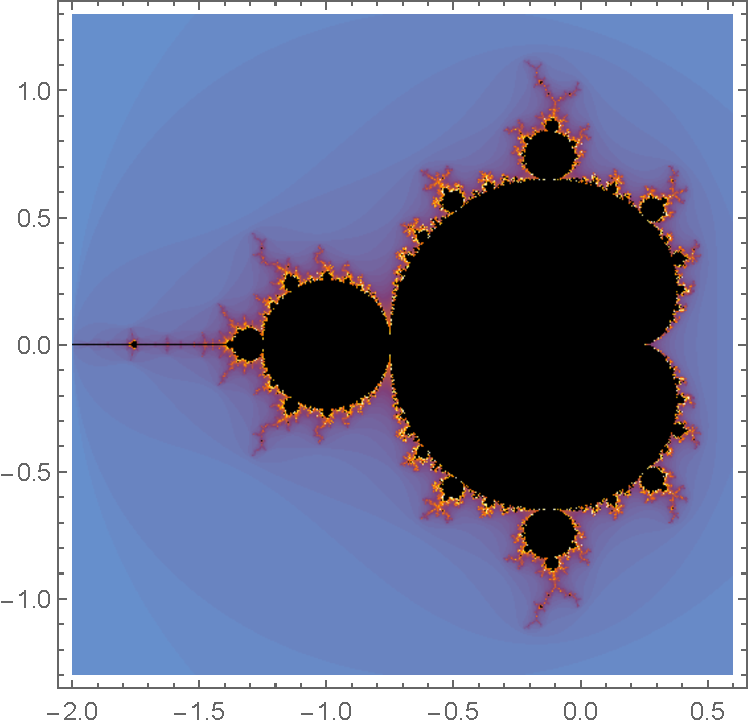
\includegraphics[width=4cm,clip]{figure.pdf}
\caption{図の挿入例}\label{サンプル図}
\end{figure}

\noindent
注意:1ページいっぱいまで書くこと(右段の下の空行が2行以下ならよい)。

\section{目的}

\section{手法}

\section{想定される成果物}

\section{進捗状況}

\section{今後の計画}

参考文献は文献ファイル(この文書では\verb|biblio.bib|)に記述し,\verb|\cite|で参照する.例:データベースのための問い合わせ言語SQLで数独を解く方法が提案されている\cite{yabuki2011}.このように参照すると,参考文献リストに自動的に登録される.文献の種類には,雑誌論文\cite{yabuki2011}や会議録論文\cite{yabuki2013},卒業論文\cite{kubo2014},書籍\cite{okumura2013},ウェブサイト\cite{self}などがある.文献の種類によって必要な項目が異なるため,\verb|biblio.bib|を見て確認すること.

\bibliographystyle{junsrt}
\bibliography{biblio}%「biblio.bib」というファイルが必要.

\end{document}
